\chapter{Desenvolvimento}
Inserindo uma figura. A figura \ref{fig:308} ilustra algum ponto importante. 
\begin{figure}[!htbp]
	\centering
	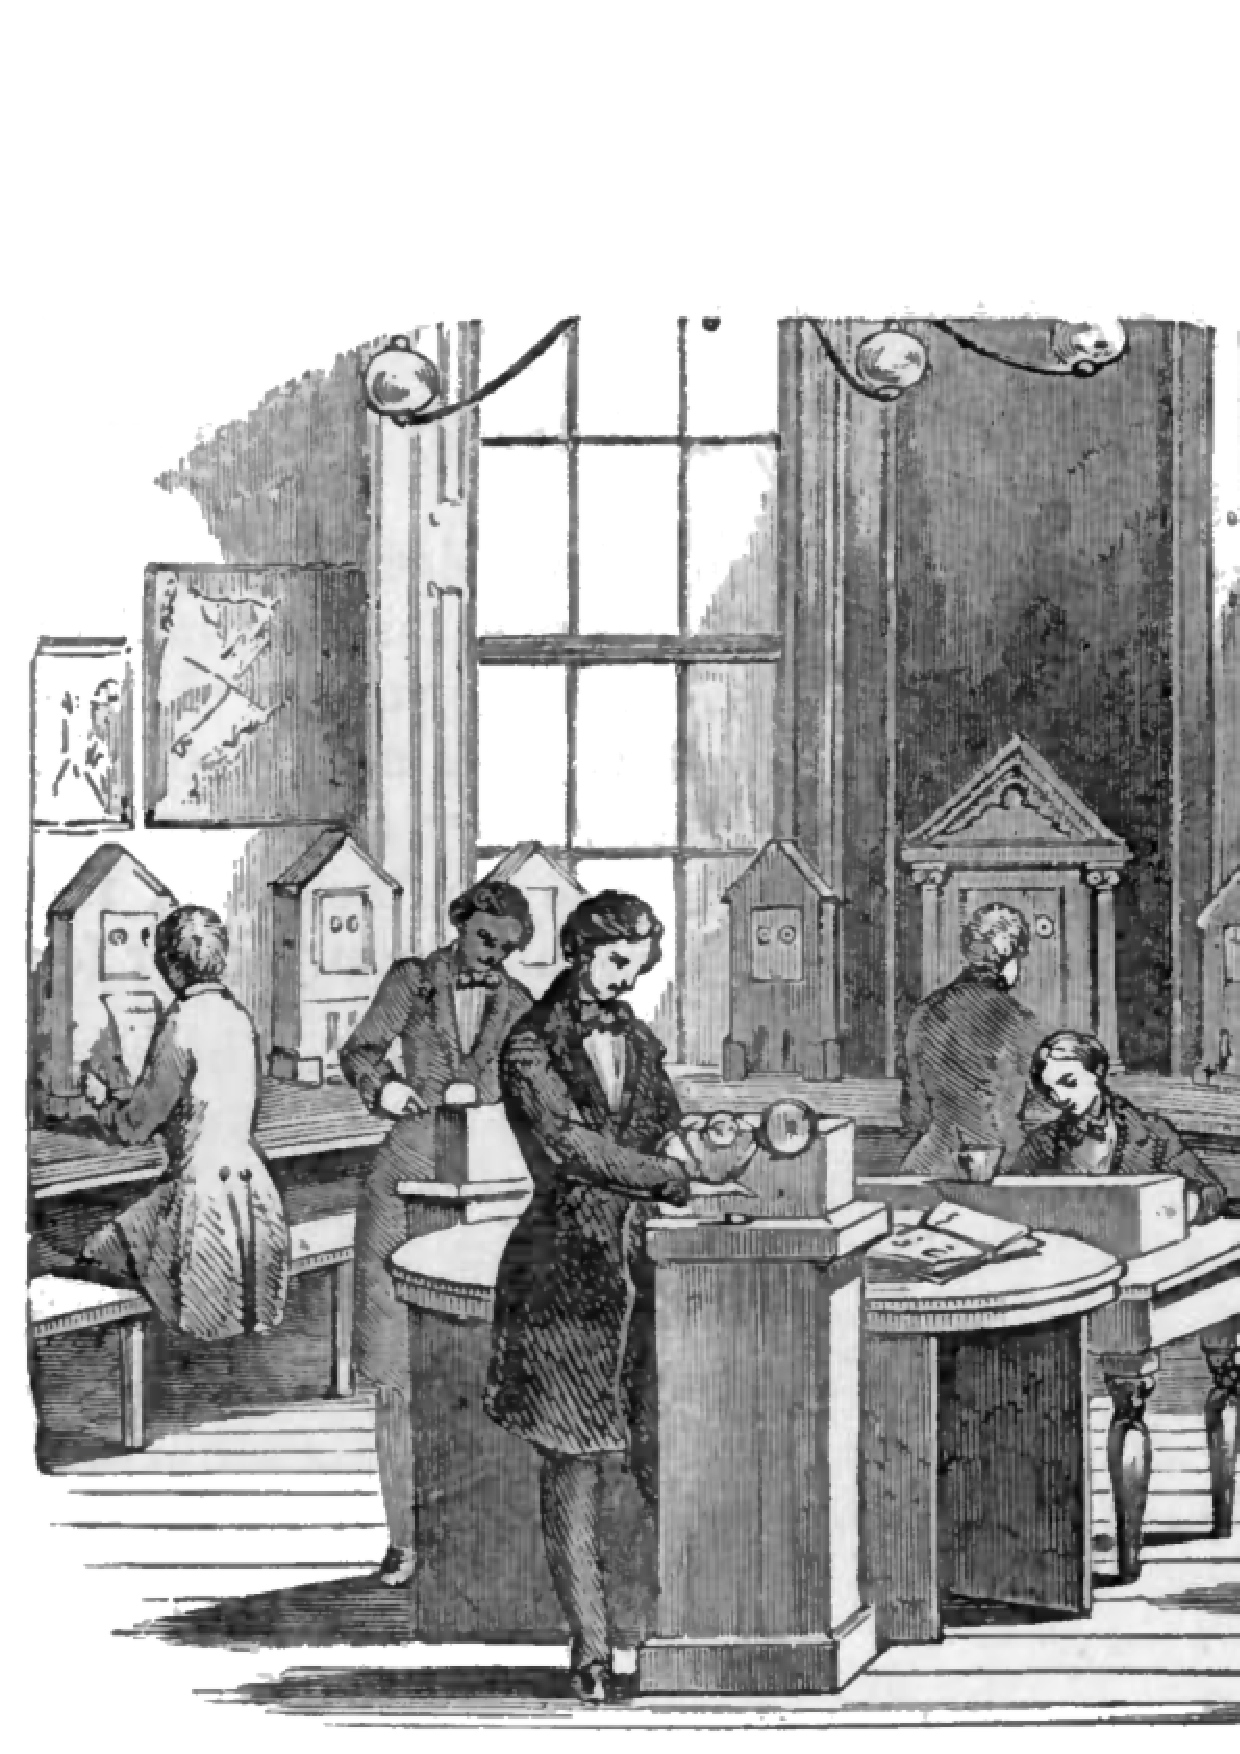
\includegraphics[scale=0.3]{figuras/fig09.pdf} % teste os valores
	\caption[Legenda reduzida - aparece no sumario]{Legenda completa. Aqui você pode colocar uma explicação melhor, sem que ela apareça no sumário do seu trabalho. Fonte: \cite[p.~117]{boyle1772}.} 
	\label{fig:308} 
\end{figure} 

Agora vem uma citação. Segundo Platão, em seu Teeteto:\footcite{platao-teeteto}
\begin{citacao}
	(...) Nam dui ligula, fringilla a, euismod sodales, sollicitudin vel, wisi. Morbi auctor lorem non justo. Nam lacus libero, pretium at, lobortis vitae, ultricies et, tellus. Donec aliquet, tortor sed accumsan bibendum, erat ligula aliquet magna, vitae ornare odio metus a mi. Morbi ac orci et nisl hendrerit mollis. Suspendisse ut massa. Cras nec ante. Pellentesque a nulla. Cum sociis natoque penatibus et magnis dis parturient montes, nascetur ridiculus mus. Aliquam tincidunt urna. Nulla
	ullamcorper vestibulum turpis. Pellentesque cursus luctus mauris.(...)
\end{citacao}

Sendo no ICHS (ver figura \ref{fig:309}, que está na página \pageref{fig:309}), teremos uma noção melhor do movimento estudantil.

\lipsum[30]

\begin{figure}[!htbp]
	\centering
	\includegraphics[scale=0.4]{figuras/ichs2.jpg} % teste os valores
	\caption[Legenda reduzida - aparece no sumario]{Legenda completa. Aqui você pode colocar uma explicação melhor, sem que ela apareça no sumário do seu trabalho. Fonte: \cite[p.~117]{boyle1772}.} 
	\label{fig:309} 
\end{figure}